This chapter describes the evolution of frame format proposed in \ref{ch:proposal}. Also, it describes the reason for each change based on better understanding the needs of the other teams and the problems in the development. Figure \ref{fig:Interface} is a diagram of our interaction with the other teams that make up this network. 
\begin{figure}[ht]
    \centering
    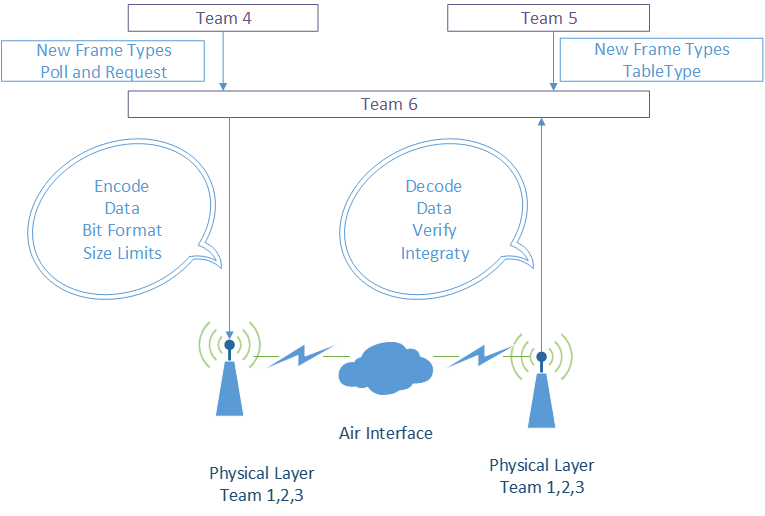
\includegraphics[width=0.8\textwidth]{Interface_diagram.PNG}
    \caption{Diagram of how Module 6 interfaces with the rest of the network}
    \label{fig:Interface}
\end{figure}


\section{MAC Frame Construction}
%TO DO Le
The proposed frame format in \ref{ch:proposal} had all the necessary fields and some removed to keep the model simple
The final frame format is  shown in \ref{tab:finalFrame}.

\begin{table}
\begin{tabular}{| c | c | c | c | c | c | c | }
  \hline                       
  Frame Type & Receiver UE & Sender UE & Data Size & Header CRC & Data & Data CRC\\
  \hline
	1 Byte & 1 Byte & 1 Byte & 1 Byte & 1 Byte & 1 to 234 Bytes & 1 Byte\\
  
  \hline  
\end{tabular}
 \caption{Final Frame Format}
	\label{tab:finalFrame}
\end{table}

\section{The transmission and reception process}
%Rebecca

Developing a frame format for transmission through the cellular network is only one part of the end-to-end requirements of data transmission. There must be a system put in place that transfers the data frame between devices and ensures that it is sent to the proper receiver. Once at the receiver, there should be a check to ensure that the data was received correctly. The reception of a correctly transmitted data frame should return a control frame, ACK, to the sender.  This allows the sending UE to be certain that the data was received correctly and allows it to resend the data frame if the ACK is not received. Just like the data frame, the ACK will have to be properly routed through the network. 

\subsection {Routing}

The network is initialized by Teams 4 and 5 who create a table of the UEs to which each BS has connected. Each UE will always transmit to the same BS, so the data frame can be automatically be sent to the initial BS in the appropriate timeslot.  To determine the routing path at the BS we need to compare the receiver ID field with the IDs in the table and identify if the receiver is connected to the initial cell or if the data frame will need to be sent between cells. If it is sent to the second BS, the data frame will undergo the same routing check again before being sent to the device specified by the receiver. The response ACK will follow the reverse path with all of the same checks at the BS(s). The path through the BSs and UEs is depicted in Figure \ref{fig:stateMachine}.

\begin{figure}[ht]
    \centering
    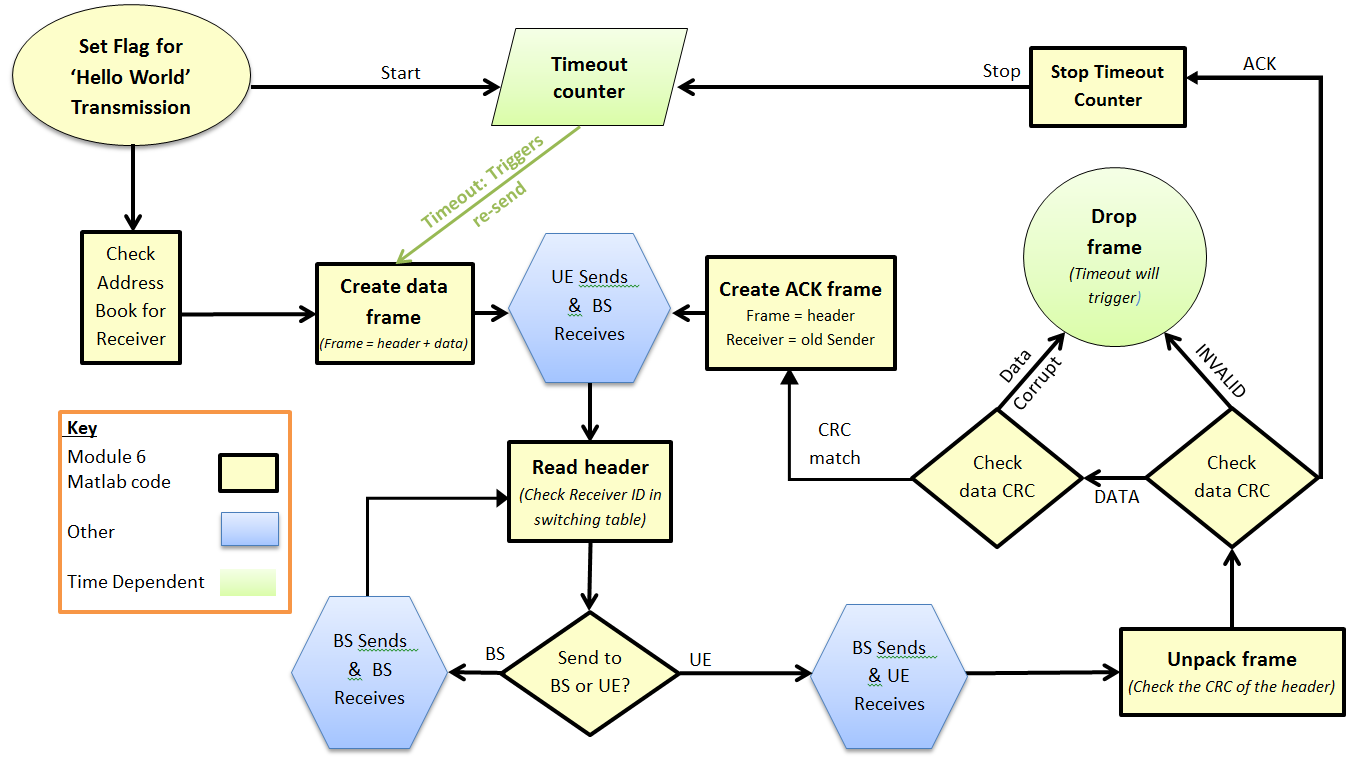
\includegraphics[width=0.9\textwidth]{State_Machine_yellow.PNG}
    \caption{State Machine of the transmission of a package }
    \label{fig:stateMachine}
\end{figure}

\subsection {The ACK response }
The ACK response should only be triggered by the transmission of correct data. We included the CRC of the data field as a section of the data frame so that the CRC can be used to check if the data has changed during any part of the transmission through the network. A data frame which fails the data CRC check will have the same result as the intended UE not receiving any frame at all or of receiving an INVALID frame: no ACK will be sent. This is shown in the Drop Frame block of Figure \ref{fig:stateMachine}. A correct data CRC should trigger the UE to send a ACK with the receiver UE ID number as the sender and the sender UE ID number as the receiver. 

If there is no ACK received back from the UE that was sent a data frame, then that data frame will eventually have to be resent from the original UE to achieve transmission. The data frame should not be resent before the ACK has an appropriate amount of time to return. Depending on the position of each UE's timeslot in the transmission cycle and whether the UEs are within the same cell, the total time between the the transmission of the data frame and the reception of the ACK will vary greatly. Figure \ref{fig:ACKtimeshort} shows the shortest possible time between transmission and reception. Figure \ref{fig:ACKtimelong} shows the longest, the time increases by a factor of 2. 

\begin{figure}[ht]
    \centering
    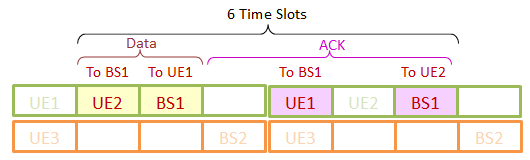
\includegraphics[width=0.6\textwidth]{ACK_timeout_short.PNG}
    \caption{Diagram of the shortest time between a UE transmitting a frame of data and receiving the corresponding ACK}
    \label{fig:ACKtimeshort}
\end{figure}

\begin{figure}[ht]
    \centering
    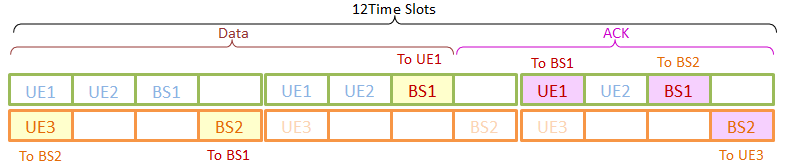
\includegraphics[width=0.9\textwidth]{ACK_timeout_long.PNG}
    \caption{Diagram of the longest time between a UE transmitting a frame of data and receiving the corresponding ACK}
    \label{fig:ACKtimelong}
\end{figure}

When the time it takes to resend a data frame is too short then there will be multiple data frames sent to the receiver even if the first transmission is received without errors. This will flood the network with at least one unnecessary data frame and ACK (if the second reception is also without error) for each data frame transmitted. When the time it takes to resend the data frame is too long the time to receive a data frame will be unnecessarily long if the transmission fails. The time it takes to resend a data frame is set to be 12 timeslots. The majority of the complete transmission times to send a data frame and receive and ACK are near 12 as can be seen in Table \ref{tab:ACKtime}. If the number of timeslots for a complete transmission was equal to or more than 10 was the exception and not the rule it might be worth it to have a lower transmission time. Unnecessary data frames and ACKs would happen rarely and would not clog the system. 

\begin{table}[ht]
	\centering
		\begin{tabular}{| c | c | c | }
		\hline                       
		Sender & Receiver & Timeslots\\
		\hline
			UE1 & UE2 & 7\\
			UE1 & UE3 & 11\\
			UE2 & UE1 & 6\\
			UE2 & UE3 & 10\\
			UE3 & UE1 & 12\\
			UE3 & UE2 & 12\\
			
		\hline
		\end{tabular}
	\caption{Table of the number of timeslots necessary to send a data frame and return an ACK for each sender and receiver}
	\label{tab:ACKtime}
\end{table}



\section{Frame Types descriptions}
%Renato
We created two frame type based on the needs of the other modules and to implement end-to-end communication.

\begin{description}
  \item[Data Frame] \hfill \\
  It is used to transmit a string message with a limit of 234 bytes. The encoding of these bytes is the ASCII standard. All the bits are ordered from the left most significant bit.
	It is important to guaranteed the decoding of this string in the receiver so that the message is not machine dependent. 
	
  \item[ACK Frame] \hfill \\
  This is the smallest package possible; it only have the header information because the data files is not transmitted. It make its transmission time smaller than any data frame. It is reused by Team 4 in their test. 
\end{description}

The frame format was designed to be used by other teams so three new types were defined by them.
\begin{description}
  \item[REQ Frame] \hfill \\
This is used by Team 4 to request a polling for all devices on the network. It is also only a header, the only difference between a request frame and an ACK is the frame type.
  \item[Poll Frame] \hfill \\
 This is used by Team 4 to return the polling information of current device and uses the data field to transmit a time in seconds. As a result of the small size, the dataSize is in bits and a CRC for the data was deemed unnecessary.
  \item[Table Frame] \hfill \\
 It is used by Team 5 to return the address table for all devices in the network. The address table is a string so this frame type is almost identical to a data frame.

\end{description} 

The frame type was a easy way to change the behavior of the receiving process based on the type.  
%RGB 253 254 202


